\chapter{Implementación del sistema de reconocimiento de gestos propuesto}\label{capit:cap4}
\vspace{-2.0325ex}%
\noindent
\rule{\textwidth}{0.5pt}
\vspace{-5.5ex}% 
\newcommand{\pushline}{\Indp}% Indent puede ir o no :p


En este cap\'itulo se describen los detalles de implementación de cada etapa del sistema.   


\section{Adquisición de los datos}\label{sec:AdquisicionDatos}

Como se vio en el capítulo \ref{capit:cap3} sección \ref{sec:KinectSensor} los datos provienen de los sensores de profundidad de dos dispositivos Kinect, estos se encuentran ubicados uno frente al usuario y otro al lado  izquierdo, con una distancia de $74$ y $79$ $cm.$ respectivamente; y entre ellos de $46$ $cm.$ como se muestra en la figura \ref{fig:SetupSystem}.
\begin{figure}[!h]
\begin{center}
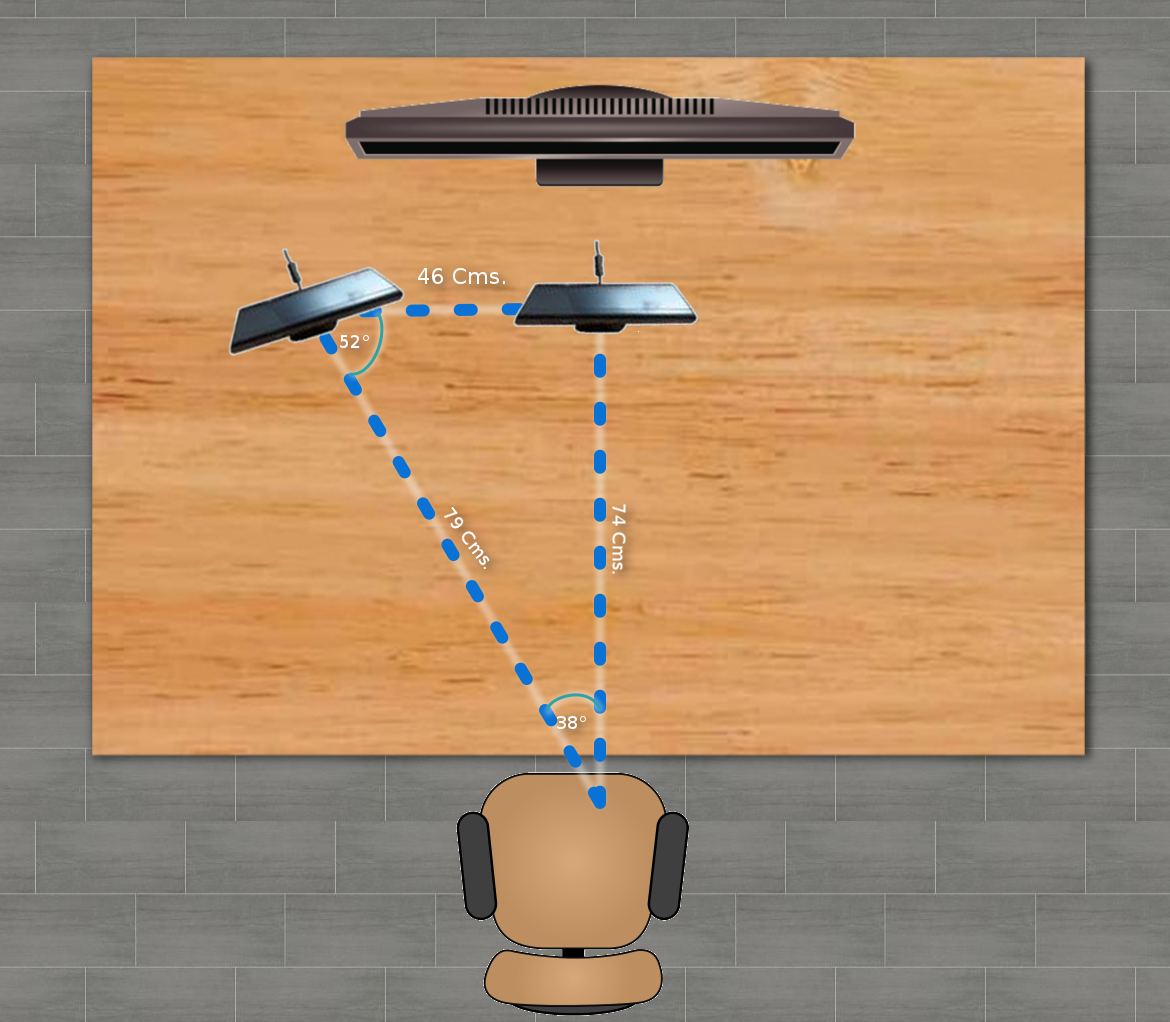
\includegraphics[scale=.2]{./Figures/system.png}
\end{center}
\caption{Configuración del sistema de reconocimiento de gestos}
\label{fig:SetupSystem}
\end{figure}  

Una vez que le flujo de datos de los sensores de profundidad es capturado este es representado como una imagen en escala de grises de $8$ bits de $640$ p\'ixeles de ancho por $480$ p\'ixeles de largo. En las imágenes se puede apreciar detalles pequeños, es decir cambios en la profundidad de hasta $1$  $mm.$ esto debido a que la escala de grises inicia cada $26$  $cm$. 
En la siguiente imagen se puede apreciar un ejemplo de las imágenes de profundidad. \ref{fig:ImagenCapturada}

\begin{figure}[h!]
\begin{center}
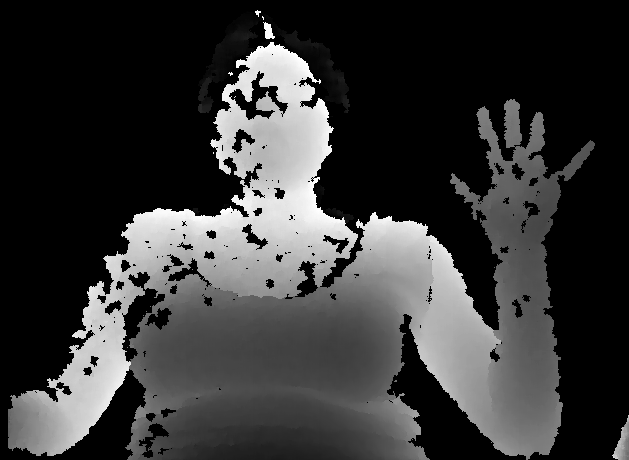
\includegraphics[scale=.5]{./Figures/166.png}
\end{center}
\caption{Representación de los datos capturados por los Kinect}
\label{fig:ImagenCapturada}
\end{figure}  

Debido a la naturaleza del funcionamiento del Kinect, las imágenes obtenidas de ambos sensores contiene ruido del tipo (poner tipo) (referencia), de manera que la imágenes provenientes de los sensores son como la figura \ref{fig:ImagenCapturadaNoNoise}; el ruido  es reducido usando filtros de mediana este es aplicado en toda la imagen usando una ventada de tamaño $13$. La imagen resultante $S(x,y)$ es como la que se muestra en la figura \ref{fig:ImagenCapturadaNoNoise}.\\ 
\begin{figure}[h!]
\begin{center}
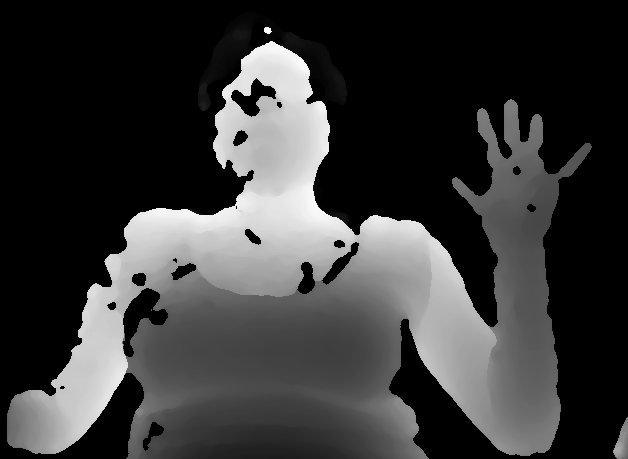
\includegraphics[scale=.5]{./Figures/166_W13.png}
\end{center}
\caption{Representación de los datos capturados por los Kinect}
\label{fig:ImagenCapturadaNoNoise}
\end{figure}  
Como se aprecia en la imagen siguiente gran parte del ruido es reducido obteniendo una mejor imagen, pero desafortunadamente todavía sigue habiendo ruido en la imagen, este puede ser eliminado casi en su mayoría  si el tamaño de la ventana aumenta pero se pierde información de la imagen de ,manera que se decidió optar por ese tamaño de ventana; la perdida de información será subsanada posteriormente. En la imagen también se aprecia el fondo negro, esto es debido a que se discrimino el fondo que estuviera a un distancia de más de $2$ $m.$ del sensor. 



\section{Detección}\label{sec:DeteccionSystem} 

En este trabajo se utiliza el algoritmo de detección de objetos desarrollado por \citep{Viola2001}, como se mostró en el cap\'itulo \ref{capit:cap3} sección \ref{subsec:ViolaJones}, el algoritmo clasifica las imágenes basándose en el valor de características, el clasificador es construido usando el algoritmo de AdaBoost en forma de cascada. 


La selección de las características se llev\'o acabo por medio de una versión modificada del algoritmo AdaBoost; la implementaci\'on se realiz\'o utilizando el software OpenCV Haar training classifier \footnote{https://github.com/mrnugget/opencv-haar-classifier-training}. Se entren\'o con $1000$ imágenes positivas (imágenes de profundidad de la mano), y $2000$ negativas, (imágenes de fondo de distintos escenarios). Las imágenes positivas fueron generadas de $100$ imágenes de la mano usando el software Create Samples \footnote{http://note.sonots.com/SciSoftware/haartraining.html}. Todas las imágenes usadas fueron tomadas de nuestra base de  datos \footnote{https://github.com/americamm}.

Nuestra base de datos contiene gran cantidad de imágenes de profundidad. Imágenes de fondo y de mano, estas fueron tomadas a una distancia de entre $60$ y $200$ $cm.$. Las imágenes de profundidad de la mano fueron tomadas de $6$ personas distintas con tres distintas poses: palma con los dedos separados \ref{fig:ImagenesPoses:2}, palma con dedos juntos \ref{fig:ImagenesPoses:3} y finalmente el pu\~no \ref{fig:ImagenesPoses:1}, como se muestran en la figura \ref{fig:ImagenesPoses}. Las imágenes de fondo fueron tomadas de distintos escenarios como se muestra en la figura \ref{fig:ImagenFondo}. El programa para la captura de las imágenes puede ser encontrado en github \footnote{https://github.com/americamm}.  

\begin{figure}[h!]
\begin{center}
\subfigure[Palma de la mano con los dedos separados.]{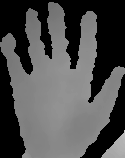
\includegraphics[scale=1]{./Figures/TrainingImage2.png}\label{fig:ImagenesPoses:2}}      \quad
\subfigure[Puño.]{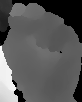
\includegraphics[scale=1.55]{./Figures/TrainingImage1.png}\label{fig:ImagenesPoses:1}}   \quad
\subfigure[Palma de la mano con los dedos juntos.]{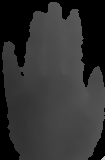
\includegraphics[scale=.99]{./Figures/TrainingImage3.png}\label{fig:ImagenesPoses:3}}
\end{center}
\caption{Ejemplo de imágenes de poses de nuestra base de datos.}
\label{fig:ImagenesPoses}
\end{figure}  

\begin{figure}[h!]
\begin{center}
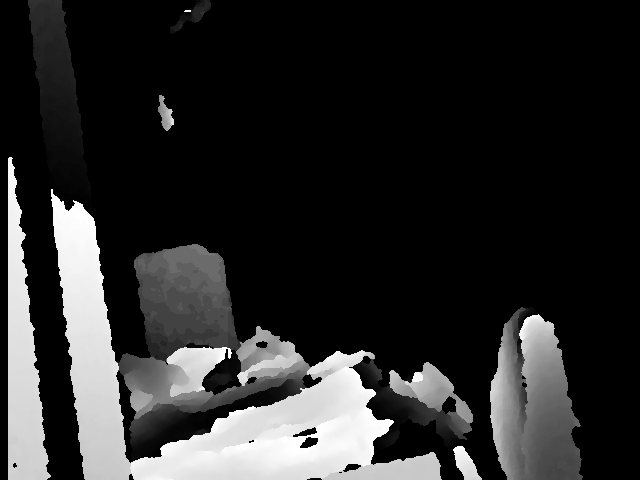
\includegraphics[scale=.4]{./Figures/Fondo5262.png}
\end{center}
\caption{Imagen del fondo de nuestra base de datos}
\label{fig:ImagenFondo}
\end{figure}  

Para localizar la mano en cada cuadro proveniente de los dispositivos  Kinect, una ventana de tamaño $ka$ se desliza por la imagen, una vez que la mano se localiza la región de interés $ROI(x,y)$ es seleccionada alrededor de la mano, como se puede ver en la figura \ref{fig:Roi}.

\begin{figure}[h!]
\begin{center}
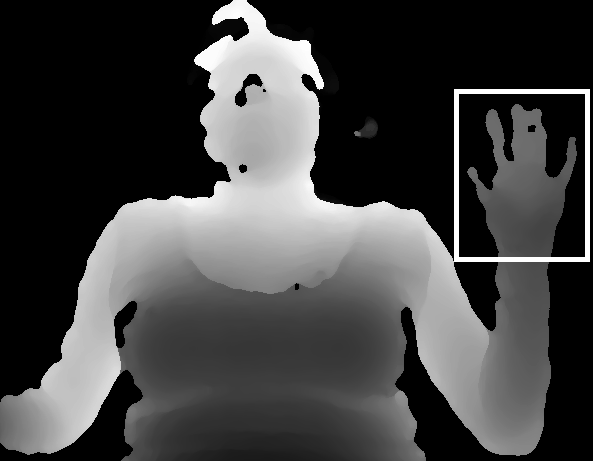
\includegraphics[scale=.5]{./Figures/roi.png}
\end{center}
\caption{Mano seleccionada}
\label{fig:Roi}
\end{figure}  

Ya que se tiene localizada el área donde se encuentra la mano, el siguiente paso es segmentar la mano del ROI. La segmentación se realiza encontrando los contornos existentes en la ROI y se toma el contorno más grande como el contorno de la mano, antes de calcular el contorno se realizan una serie de procesamientos al ROI para eliminar ruido y que el cálculo del contorno sea más preciso.    

El primer procesamiento que se aplica al ROI, son las operaciones morfológicas: apertura y cierre, en ese orden. Se utilizan para eliminar uniones pequeñas que existen en la imagen como el de la figura \ref{fig:RuidoUnion} o unir pequeños hoyos que existen en la imagen, como los que se encuentran en la figura \ref{fig:RuidoHoyo}.\\
Las operaciones anteriores utilizan un elemento estructural rectangular; para la operación de apertura el tamaño del elemento es de $3 \, x \, 7$ pixeles; para el cierre se aplic\'o con un tamaño  $7 \, x \, 7$ pixeles.\\
\begin{figure}[h!]
\begin{center}

\includegraphics[scale=.5]{./Figures/pusheen.png}
\end{center}
\caption{ROI que muestra una unión entre los dedos}
\label{fig:RuidoUnion}
\end{figure}   
\begin{figure}[h!]
\begin{center}

\includegraphics[scale=.5]{./Figures/pusheen.png}
\end{center}
\caption{ROI donde se aprecio un hoyo en la mano}
\label{fig:RuidoHoyo}
\end{figure}  
Las imágenes siguientes muestran el resultado de aplicar las operaciones apertura y cierre al ROI. 
\begin{figure}[h!]
\begin{center}

\includegraphics[scale=.5]{./Figures/pusheen.png}
\end{center}
\caption{Apertura y cerradura}
\label{fig:ImagenOpenClose}
\end{figure}  

Una vez aplicadas las operaciones morfológicas el siguiente paso es binarizar la región de interés, se lleva acabo aplicando el algoritmo desarrollado por \citep{Niblack1985}, se decidió usar este método debido a la naturaleza de la imagen. Los parámetros que fueron usados fueron $k=0.5$ y una ventana de $3x3$ p\'ixeles. La figura siguiente es la imagen binarizada. 

\begin{figure}[h!]
\begin{center}

\includegraphics[scale=.5]{./Figures/pusheen.png}
\end{center}
\caption{Binarización de ROI}
\label{fig:BinarizationRoi}
\end{figure}
 
Cuando la ROI es binarizada el siguiente paso es encontrar los contornos existentes dentro del ROI. Los contornos se calcularon utilizando el algoritmo de $blabla$ con tales parámetros. La fig. \ref{fig:ImageHandContour} muestra en color blabla el contorno de la mano. 

\begin{figure}[!h]
\begin{center}

\includegraphics[scale=.5]{./Figures/pusheen.png}
\end{center}
\caption{Contorno de la mano}
\label{fig:ImageHandContour}
\end{figure}
  


\section{Extracción de características}\label{sec:ExtraccionCaracteristicasSystem}

Como se vio en el capítulo \ref{capit:cap3} sección \ref{sec:Convexhull} las características de la mano son extraídas utilizando los algoritmos de envolvente convexa y  defectos de convexidad.\\
La figura muestra un ejemplo de la aplicación de estos algoritmos al ROI.  

\begin{figure}[!h]
\begin{center}

\includegraphics[scale=.5]{./Figures/pusheen.png}
\end{center}
\caption{En esta dibujado el casco convexo los punto en son los defectos de convexidad}
\label{fig:Convex&Defects}
\end{figure}


Una vez aplicados estos dos algoritmos se pueden calcular el número de dedos y las puntas de estos que son fundamentales para calcular las demás características. Enseguida se describe el algoritmo \ref{alg:NumDedos} para calcular el número de dedos.\\ 
Sea $CD=\lbrace cd_1, cd_2, \cdots, cd_n \rbrace$ los defectos de convexidad de una envolvente convexa. Cada defecto esta compuesto de tres elementos $\lbrace s_i(x,y),d_i(x,y),e_i(x,y) \rbrace \in cd_i, \quad i=\lbrace 1, 2, \cdots, n\rbrace$. Sea $D$ el conjunto de las distancias de $d_i(x,y)$ a la orilla de la envolvente convexa.  

\begin{algorithm}
\begin{algorithmic}[1]

\REQUIRE $D=\lbrace \delta_1, \delta_2, \cdots, \delta_n \rbrace$.  
\ENSURE Número de dedos, $Nf$.  

\FOR{$i=1$ hasta $n$}  
	\STATE $minDist=20$, $maxAng=60$, $antecesor=0$, $sucesor=0$. 	
	
	\IF{$\delta_i < minDepth$ } 
	\STATE continuar
	\ENDIF 
	
	\IF{i=0} 
	\STATE $antecesor=n-1$
	\ELSE
	\STATE $antecesor=i-1$
	\ENDIF 

	\IF{i=n-1} 
	\STATE $sucesor=0$
	\ELSE
	\STATE $sucesor=i+1$
	\ENDIF   
	
	\STATE Calcular el $angulo$ entre $s_{antecesor}(x,y)$ y $s_{sucesor}(x,y)$
	
	\IF{$angulo \geqslant maxAng$}
	\RETURN \FALSE
	\ENDIF  
	
	\STATE $Nf=Nf+1$.

\ENDFOR 
\caption{Calcula el número de dedos de la mano.}
\label{alg:NumDedos}
\end{algorithmic}
\end{algorithm}

El ángulo $\alpha$ entre los dedos $f_j$ y $f_{j+1}$ es calculado como:  
$$ \alpha_{f_j} = \tan^{-1}{ \bigg| \frac{m_{j+1}-m_j}{1+m_{j+1}m_j} \bigg|}$$
donde $m_{j+1},m_j$ son las pendientes de las rectas que pasa por los puntos $d_j(x,y)$ y $s_{j+1}(x,y)$; $d_j(x,y)$ y $s_j(x,y)$; $j=\lbrace 1,2,3,4,5 \rbrace$.  

El ángulo del centro de la mano a la punta de los dedos puede ser obtenido como: 
$$ \theta_{f_j} = \tan^{-1} | {m_j} - 90^\circ |$$
donde $m_j$ es la pendiente de la recta que pasa por el centro de la mano y la punta de los dedos $s_i(x,y)$.

Las características se guardan en un vector de características de dimensión $26$.



\section{Reconocimiento}\label{sec:ReconocimientoSystem}

En este trabajo se reconocen gestos estáticos y dinámicos utilizando el algoritmo de clasificación de máquina de soporte vectorial.  

Como se vio en el capitulo \ref{capit:cap3} sección \ref{sec:SVM} SVM es un algoritmo de aprendizaje de máquina supervisado, por lo que es necesario tener imágenes de los gestos a reconocer ya que con estas el clasificador es entrenado y el modelo de clasificación puede ser creado. 

La implementación de SVM se lleva acabo usando LibSVMSharp \footnote{https://github.com/ccerhan/LibSVMsharp} un wrapper de la librería LibSVM \citep{Chang2011}.

\subsection{Reconocimiento de gestos estáticos}\label{RecognitionEstatic}

El sistema reconoce dos gestos estáticos: el puño y la palma de la mano con los dedos separados.  Para el entrenamiento se tomaron $num$ imágenes de los dos distintos gestos como los de la fig \ref{fig:SVMTrainingStatic}, divididas en partes iguales. De tamaño $640$ por $480$ pixeles.   

\begin{figure}[h!]
\begin{center}
\subfigure[Palma de la mano con los dedos separados.]{
\includegraphics[scale=.5]{./Figures/pusheen.png}\label{fig:SVMTrainingStatic:1}}      \quad
\subfigure[Puño.]{
\includegraphics[scale=.5]{./Figures/pusheen.png}\label{fig:SVMTrainingStatic:2}}
\end{center}
\caption{Ejemplo de imágenes de poses de nuestra base de datos.}
\label{fig:SVMTrainingStatic}
\end{figure}

Para el entrenamiento de la máquina de soporte se utilizo un kernel exponencial, (poner los demás parámetros) y se utilizó validación cruzada con 5 pliegues. 

\subsection{Reconocimiento de gestos dinámicos}\label{RecognitionDynamic}

El sistema reconoce numero de gestos dinámicos.  

%\subsection{Extracción de parámetros}
%Ecuación \ref{eq:gravedad}. 
%
%\begin{equation} \label{eq:gravedad}
%A_{d} = -g - \frac{\sum F}{mass}
%\end{equation} 

%Donde $A_{d}$ representan la aceleración que se aplica a un dispositivo, $g$ la constante de gravedad de 9.81 m/$s^{2}$, y $\sum F$ las fuerzas que se aplican al propia sensor.

%Text  \ref{eq:demandaOxigeno_personalizada} and more $O_{2}$ text:
%
%\begin{equation} \label{eq:demandaOxigeno_personalizada}
%\begin{split} 
%& K = R + H + V \\ 
%& R = 3.5 - (0.0367 \times BMI) - (0.0038 \times age) + (0.1790 \times gender)\\
%& H = 0.1 \times \textrm{velocidad de desplazamiento}\\ 
%& V = 1.8 \times \textrm{velocidad de desplazamiento}\\ 
%\end{split} 
%\end{equation} 
%
%Donde $1 + 2$ representan el consumo de $O_{2}$ en reposo personalizado al usuario $(ml \times kg^{-1} \times min^{-1})$ \citep{Barstow:1991}, $H$ el componente horizontal relativo a la velocidad de desplazamiento (m/min), $V$ el componente vertical relativo a la velocidad (m/min) y pendiente de desplazamiento (\%).
%
%\begin{description}
%  \item[Velocidad:] \hfill \\
%  	Para obtener la velocidad de desplazamiento se utiliza el número de pasos realizados por el usuario como se muestra a continuación (Ecuación \ref{eq:velocidad}).
%  
%\begin{equation} \label{eq:velocidad}
%  S_{k} = D_{k}/W \hspace{10 mm} 
%  D_{k} = ST_{k} \times SL \hspace{10 mm}
%  SL = D_{total}/ST_{total} 
%\end{equation}
%\end{description}
	
\newpage
%%=====================================================

